%%% LaTeX Template: Designer's CV
%%%
%%% Source: http://www.howtotex.com/
%%% Feel free to distribute this template, but please keep the referal to HowToTeX.com.
%%% Date: March 2012


%%%%%%%%%%%%%%%%%%%%%%%%%%%%%%%%%%%%%
% Document properties and packages
%%%%%%%%%%%%%%%%%%%%%%%%%%%%%%%%%%%%%
\documentclass[letterpaper,12pt,final]{memoir}

% misc
\renewcommand{\familydefault}{bch}	% font
\pagestyle{empty}					% no pagenumbering
\setlength{\parindent}{0pt}			% no paragraph indentation


% required packages (add your own)
\usepackage{flowfram}										% column layout
\usepackage[top=1cm,left=0.2cm,right=1cm,bottom=0.8cm]{geometry}% margins
\usepackage{graphicx}
\usepackage{epstopdf} 									% figures
\usepackage{url}											% URLs
\usepackage[usenames,dvipsnames]{xcolor}					% color
\usepackage{multicol}										% columns env.
	\setlength{\multicolsep}{1pt}
\usepackage{paralist}										% compact lists
\usepackage{tikz}
\usepackage{textcomp}
\usepackage{amsmath,amsfonts}
%\usepackage[none]{hyphenat}
\usepackage{geometry}
\geometry{
	%letterpaper,
	%total={215.9mm,279.4mm},
	left=8mm,
	right=18mm,
	%top=7mm,
	%bottom=7mm,
}

%\usepackage{anyfontsize}
\usepackage[hidelinks]{hyperref}
\usepackage[pscoord]{eso-pic}% The zero point of the coordinate systemis the lower left corner of the page (the default).
\usepackage{xcolor}

%%%%%%%%%%%%%%%%%%%%%%%%%%%%%%%%%%%%%
% Create column layout
%%%%%%%%%%%%%%%%%%%%%%%%%%%%%%%%%%%%%
% define length commands
\righthyphenmin =62
\lefthyphenmin =62

\setlength{\vcolumnsep}{\baselineskip}
\setlength{\columnsep}{\vcolumnsep}

% frame setup (flowfram package)
% left frame
\newflowframe{0.265\textwidth}{\textheight}{0pt}{0pt}[left]
	\newlength{\LeftMainSep}
	\setlength{\LeftMainSep}{0.21\textwidth}
	\addtolength{\LeftMainSep}{4\columnsep}

%\renewcommand{\ffvrule}[3]{%
%	\hfill
%	\tikz{\draw[loosely dotted,color=Plum,line width=1.5pt,yshift=0](0,0) -- (0,0);}
%	\hfill\mbox{}}
%\insertvrule{flow}{1}{flow}{2}

% right frame
\newflowframe{0.7\textwidth}{\textheight}{\LeftMainSep}{0pt}[main01]

% horizontal rule between frames (using TikZ)
\renewcommand{\ffvrule}[3]{%
\hfill
\tikz{\draw[loosely dotted,color=Plum,line width=1.5pt,yshift=-#1](0,0) -- (0,#3);}
\hfill\mbox{}}
\insertvrule{flow}{1}{flow}{2}

%%%%%%%%%%%%%%%%%%%%%%%%%%%%%%%%%%%%%
% define macros (for convience)
%%%%%%%%%%%%%%%%%%%%%%%%%%%%%%%%%%%%%
\newcommand{\Sep}{\vspace{1.5em}}
\newcommand{\SmallSep}{\vspace{0.5em}}

\newenvironment{Objective}
	{\ignorespaces\textbf{\color{Plum} Objective}}
	{\Sep\ignorespacesafterend}
	
\newcommand{\CVSection}[1]
	{\Large\textbf{\textsc{{#1}}}\par
	\SmallSep\normalsize\normalfont}

\newcommand{\CVItem}[1]
	{\textsc{\color{Plum} #1}}

\newcommand{\CVItemSC}[1]
{{\textsc{\color{Plum} #1}}}

\newcommand{\placetextbox}[3]{% \placetextbox{<horizontal pos>}{<vertical pos>}{<stuff>}
	\setbox0=\hbox{#3}% Put <stuff> in a box
	\AddToShipoutPictureFG*{% Add <stuff> to current page foreground
		\put(\LenToUnit{#1\paperwidth},\LenToUnit{#2\paperheight}){\vtop{{\null}\makebox[0pt][c]{#3}}}%
	}%
}%

\newcommand{\plumBox}[1]
{\space\space\colorbox{Plum!10}{\tiny \textbf{{#1}}}}

\newcommand{\RightAlignedInlineText}[1]
{{\footnotesize \color{Plum}  \hfill [#1]}}

%%%%%%%%%%%%%%%%%%%%%%%%%%%%%%%%%%%%%
% Begin document
%%%%%%%%%%%%%%%%%%%%%%%%%%%%%%%%%%%%%
\begin{document}

% Left frame
%%%%%%%%%%%%%%%%%%%%
%\begin{figure} 
%	\hfill
%	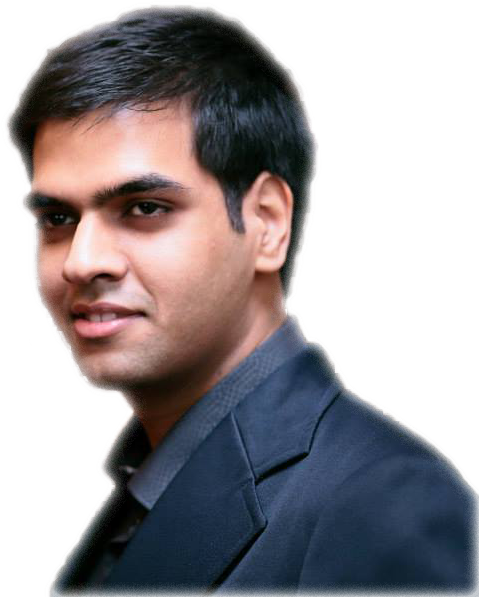
\includegraphics[width=0.8\columnwidth]{kkk}
%	\vspace{-5cm}
%\end{figure}

\begin{flushright} 
	\footnotesize
	\SmallSep
	\CVItemSC{Address}\\%{\bfseries{\color{Plum}{Address}}}\\
	
	2500, Avent Ferry Rd.\\
	Apartment No. 205\\
	Raleigh, NC - 27606\\
	\Sep
	\CVItemSC{E-Mail}\\%{\bfseries{\color{Plum}{E-Mail}}}\\
	\href{mailto:vicky.p.katara@gmail.com}{\texttt{vicky.p.katara@gmail.com}}\\
	\Sep
	\CVItemSC{Mobile}\\%{\bfseries{\color{Plum}{Cellphone}}}\\
	\href{tel:+19842158067}{+1 984 215 8067}\\
	\SmallSep
		%{\bfseries{\color{Plum}{Website}}}\\
	%\href{http://vickykatara.orgfree.com/}{vickykatara.orgfree.com}\\
	\Sep
	\CVItemSC{GitHub Repo}\\%{\bfseries{\color{Plum}{Cellphone}}}\\
	\href{https://github.com/vicky-katara}{\texttt{github.com/vicky-katara}}\\
	\SmallSep
		\tikz{\draw[loosely dotted,color=Plum,line width=1.5pt](6.2,0) -- (1,0);}
%\end{flushright}\normalsize	
\SmallSep
\CVSection{Skills}
\CVItemSC{Programming Languages}\\
{\footnotesize Java, C, Python, Ruby, Rust, Excel VBA}
\SmallSep\\
\CVItemSC{Web Technologies}\\
{\footnotesize HTML, CSS, JavaScript, XML}
\SmallSep\\
\CVItemSC{Database Platforms}\\
{\footnotesize Advanced SQL on Oracle RDBMS 9i / 11g}
\SmallSep\\
\CVItemSC{Applications}\\
{\footnotesize Informatica PowerCenter, Adobe Photoshop CS6, NetBeans, Eclipse, Audacity, \LaTeX, Wireshark, GitHub, Swing(Java)}
\SmallSep\\
\CVItemSC{Operating Systems}\\
{\footnotesize Microsoft Windows, Linux}
\SmallSep\\
\CVItemSC{Certifications}\\
{\footnotesize Oracle Certified Java SE6 Programmer\space(with 93\%)}
%\SmallSep
%\end{flushright}\normalsize
%\SmallSep\\
%\Sep\\
\end{flushright}\normalsize
\tikz{\draw[loosely dotted,color=Plum,line width=1.5pt](6.2,0) -- (1,0);}
\SmallSep
%\begin{figure}
	%\hfill
	%\vspace{-0.3cm}
	\hspace{0.7cm}
		\vspace{-0.35cm}
	\textsc{\bfseries{\color{Plum}{Save My Contact}}}\\\\
	\vspace{+0.45cm}
	%\hspace{-0.4cm}
	
\includegraphics[width=0.8\columnwidth]{qrcode_2.eps}
%\end{figure}
\framebreak

% Right frame
%%%%%%%%%%%%%%%%%%%%
%\rhead{Last Updated: Jan 16, 2016}
\placetextbox{0.88}{0.995}{\color{Plum}\footnotesize{Last Updated: Jan 31, 2016}}%
\Huge\bfseries \textsc{\color{Plum} Vicky Katara} 
%\Large\bfseries  Graduate Computer Science Student 
\SmallSep

\normalsize\normalfont

% About me
%\begin{Objective}
%\\Achieve excellence in the field of Computer Science while refining the ability of visualization and rationality of thought.
%\end{Objective}

% Education
\CVSection{Education}
\CVItem{2015 - 2017 (Expected), M.S.(Computer Science),\\ North \hyphenchar\font=-1 Carolina State University}\\
\begin{footnotesize}
	Current G.P.A.: 4.0
\end{footnotesize}
\SmallSep

\CVItem{2009 - 2013, B.E.(Computer Engineering), University of \allowbreak  Mumbai}\\
 \begin{footnotesize}
 	Majored in Software / Computer Science. Graduated 6th in class.
 \end{footnotesize}
\SmallSep

% Experience
\CVSection{Work Experience}
\CVItem{Jan 2014 \textendash \space Jun 2015, Technology Analyst, Deloitte Consulting}\\
\SmallSep
Business Intelligence - Data Warehousing\\
{\footnotesize Optimized prevalent processes by building automation tools. Inspired rethinking of existing problem solving strategies in Business Intelligence and Data Warehousing while discovering unexplored risk mitigation policies. Initiated and lead numerous social responsibility projects.}
\SmallSep

% Projects - Start
\CVSection{Relevant Projects}
%Project-new1 Start
\CVItem{Conformance Suite for Mozilla Servo} \RightAlignedInlineText{Sept-Dec 2015}\\
{\footnotesize Open Source project to develop a conformance suite for Mozilla's next generation browser. Source at: \color{Plum} \href{https://github.com/vicky-katara/unicode-bidi}{\space\space\texttt{vicky-katara/unicode-bidi}} \\\color{Black}
	\emph{Technologies Used:} Python, Rust}%Project-4 End
\SmallSep\\
%Project-new1 Start
\CVItem{Peer to Peer Video Streaming System} \RightAlignedInlineText{Oct-Dec 2015}\\
{\footnotesize Developed a P2P Video Streaming Application. Source at: \color{Plum} \href{https://github.com/vicky-katara/IP_Video_P2P.git}{\space\space\texttt{vicky-katara/IP\_Video\_P2P}} \\\color{Black}
	\emph{Technologies Used:} Java, Eclipse, testing on a VirtualBox swarm}%Project-4 End
\SmallSep\\
\CVItem{Java File Encryptor} \plumBox{Side Project} \RightAlignedInlineText{Jan 2015}\\
{\footnotesize My attempt at Building a File Encryption Tool in Java. The GUI is in Swing. It uses PBE with MD5 and DES for encryption. Source at: \color{Plum} \href{https://github.com/vicky-katara/FileEncryptor.git}{\space\space\texttt{vicky-katara/FileEncryptor}} \\\color{Black}
	\emph{Technologies Used:} Java, Swing, NetBeans}%Project-4 End
\SmallSep\\
%Project-new1 Start
\CVItem{Library Management System}\RightAlignedInlineText{Sept-Oct 2015}\\
{\footnotesize Modeled and developed a Library Management System as a Web Application. \\Application available at: \color{Plum} \href{https://calm-coast-3120.herokuapp.com/}{\space\space\texttt{calm-coast-3120.herokuapp.com}} \\\color{Black}
	\emph{Technologies Used:} Ruby on Rails, CSS, JavaScript, Heroku}%Project-4 End
\SmallSep\\
\CVItem{GRE Word Test tool}\plumBox{Side Project} \RightAlignedInlineText{Sep 20, 2015}\\
{\footnotesize Application available at: \color{Plum} \href{http://www4.ncsu.edu/~vpkatara/GRE800/}{\space\space\url{www4.ncsu.edu/ ~vpkatara/GRE800/}} \\\color{Black}
	\emph{Technologies Used:} JavaScript, HTML, CSS}%Project-4 End
\SmallSep\\
%Project-4 Start
\CVItem{Analysis of Atomicity for Multithreaded Programs} \RightAlignedInlineText{July-Dec 2012}\\
{\footnotesize Researched into algorithms for testing atomicity(serializability) of multi-threaded programs. Implemented live applications to test the results. emph{\\Technologies Used:} Java, Swing, NetBeans}%Project-4 End
\SmallSep\\
\CVItem{Warehouse Testing Automator} \plumBox{Side Project} \RightAlignedInlineText{March-Dec 2014}\\
{\footnotesize Developed a tool to execute SQL Test scripts on a database, capture the results, and publish them onto an Auditing and Testing platform. The tool is currently being patented by Deloitte.\\ \emph{Technologies Used:} Microsoft VBA, SQL} 
%Project-5 Start
%\CVItem{Development of Mini-Tennis Game, Mini-Project for Computer Graphics}\\
%{\footnotesize This involved the design and development of 2D Mini-Tennis game.\\ \emph{Technologies Used:} GCC}\\%Project-5 End
%\Sep 
% Projects - End
%%%%%%%%%%%%%%%%%%%%%%%%%%%%%%%%%%%%%
% End document
%%%%%%%%%%%%%%%%%%%%%%%%%%%%%%%%%%%%%
\end{document}